\subsection{Opsamling af accelerometersignaler}

Accelerometrene testes for at vurdere, hvorvidt de opstillede krav i \autoref{sec:acc_teori} opfyldes. 
Det fremgår af databladet, at accelerometrene er triaksiale.  
Ud fra målinger, foretaget i \autoref{sec:test_acc}, ses en lineær tendens med en afvigelse på gennemsnitlig $2~\%$, hvilket derfor lever op til kravet for lineariteten. 
Da det ikke er muligt at teste, om accelerometrene har accelerationer i $\pm2~g$, tages der udgangspunkt i databladet. 
I databladet beskrives det, at accelerometrene har et lineært arbejdsområde på $\pm 3~g$.
Accelerometrene kan, ud fra databladet, forsynes med en DC-forsyning fra $1,8-3,6~V$ \citep{analogdevices2009}.  
Det er derfor testet, hvorvidt mikrokontrolleren forsyner accelerometrene med en spænding indenfor dette område. 
Testen er udført ved brug af et multimeter, hvortil der måles en spænding på $3,2~V$. 
Test af mikrokontrolleren er udført i \autoref{sec:samlet_system}, hvorved kravet om en spænding mellem $1,8$ og $3,6~V$ er opfyldt.

\vspace{3mm}
\textbf{Opsummering af krav:}
\begin{itemize}
\item[\text{\sffamily \checkmark}] Skal måle på minimum én akse
\item[\text{\sffamily \checkmark}] Skal have en linearitet med en afvigelse på $5\%$
\item[\text{\sffamily \checkmark}] Skal måle accelerationer i $\pm2~g$
\item[\text{\sffamily \checkmark}] Skal forsynes med en spænding mellem $1,8$ og $3,6~V$
\end{itemize}


\subsection{Opsamling og behandling af EMG-signaler}

EMG-forstærkeren testes for at vurdere, hvorvidt der kan opsamles muskelaktivitet fra rectus femoris. 
Overfladeelektroderne placeres ud fra SENIAM's anvisning om elektrodeplacering, jf. \autoref{sec:pilotforsoeg}. 
En squat-øvelse udføres, hvorefter muskelsignaler A/D-konverters ved brug af mikrokontrolleren og visualiseres i MATLAB. 
Denne øvelse er beskrevet i \autoref{sec:knaeled_squat}. 
Muskelsignalet, under udførslen af squat-øvelsen, fremgår af \autoref{fig:raat_emg}. 

\begin{figure}[H]
\centering
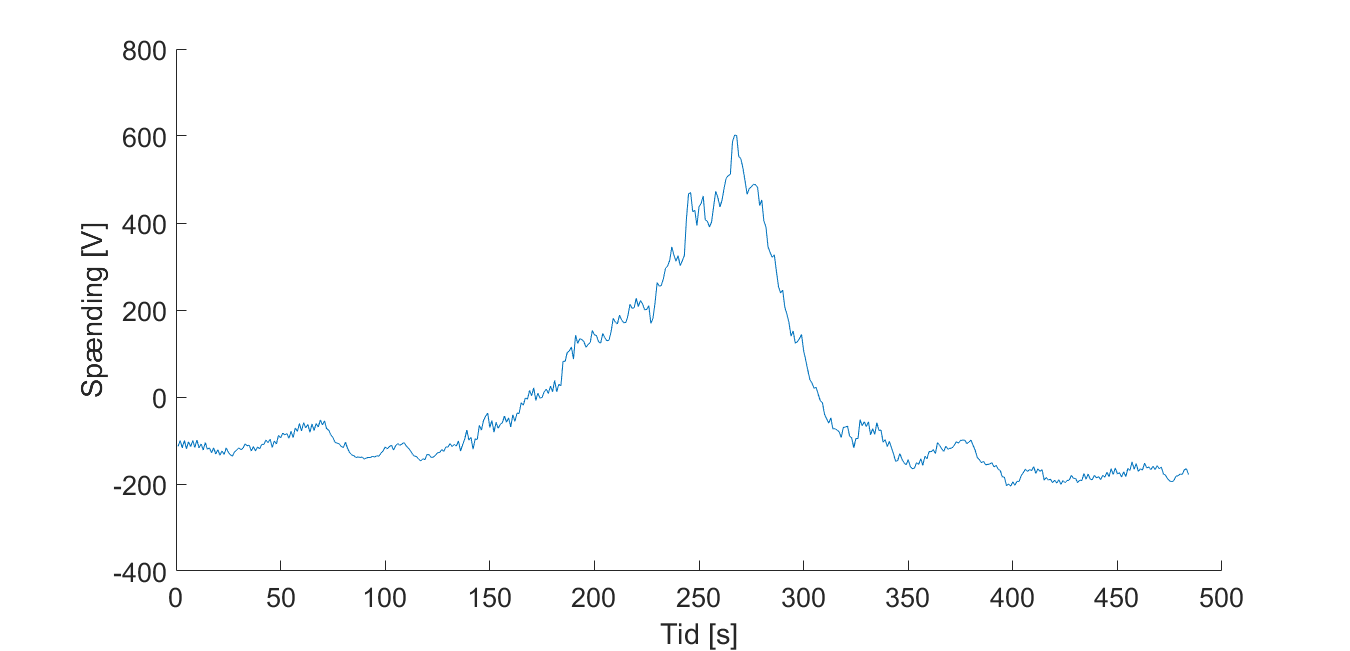
\includegraphics[width=1\textwidth]{figures/raat_EMG_test}
\caption{Et samplet EMG-signal fra rectus femoris under udførsel af en squat-øvelse.}
\label{fig:raat_emg}
\end{figure}

\noindent
Ud fra \autoref{fig:raat_emg} ses den opsamlede muskelaktivitet fra rectus femoris. 
For således at undersøge, hvorvidt muskelsignalerne ligger i frekvensområdet mellem $10-500~Hz$, er en frekvensanalyse foretaget. 
Grundet EMG-forstærkerens virkemåde forventes det, at frekvensområdet er mere lavfrekvent, da det envelopefiltreres. 
Dette fremgår ligeledes af frekvensanalysen, foretaget i \autoref{sec:pilotforsoeg}, hvor frekvensområdet vurderes til at ligge mellem $0,4-10~Hz$. 
Hertil fortages yderligere en frekvensanalyse af signalet, der ses i \autoref{fig:raat_emg}. Frekvensanalysen fremgår af \autoref{fig:fft_raat_emg}.

\begin{figure}[H]
\centering
\includegraphics[width=1\textwidth]{figures/fft_raat_EMG}
\caption{Frekvensanalyse af samplet EMG-signal under en squat-øvelse, hvor Y-aksen er en semilogaritmisk skala.}
\label{fig:fft_raat_emg}
\end{figure}

\noindent
Frekvensanalysen sammenlignes med frekvensanalysen, der er foretaget i \autoref{sec:pilotforsoeg}, hvortil der ikke ses nogen forskel. 
Det ses af \autoref{fig:raat_emg}, at der forekommer udslag i EMG-signalet fra EMG-forstærkeren idet musklen kontraherer. Ud fra dette anses kravet om opsamling af muskelsignaler mellem $10-500~Hz$ som værende opfyldt. 

EMG-forstærkeren forsynes med en spænding på $\pm 5,4~V$, hvilket er testet i \autoref{test_spaendingsforsyning} og derved overholdes kravet om minimum spænding på $\pm 5~V$.
På EMG-forstærkeren er der et justerbart gain, således forstærkningen kan tilpasses den enkelte bruger af systemet. Ud fra dette og \autoref{fig:raat_emg} vurderes det, at EMG-forstærkeren opfylder de opstillede krav i \autoref{sec:EMG_krav}.

\vspace{3mm}
\textbf{Opsummering af krav:}
\begin{itemize}
\item[\text{\sffamily \checkmark}] Skal være anvendeligt med overflade elektroder
\item[\text{\sffamily $\div$}] Skal opsamle muskelsignaler i frekvensområdet mellem $10$ og $500~Hz$
\begin{itemize}
\item[\text{\sffamily \checkmark}] Grundet EMG-forstærkerens virkemåder bliver outputsignalet lavfrekvent, hvortil frekvensområdet er aflæst til at være mellem $0,4-10~Hz$
\end{itemize}
\item[\text{\sffamily \checkmark}] Skal forsynes med minimum en spænding på $\pm5~V$
\item[\text{\sffamily \checkmark}] Skal have et justerbart gain, der kan tilpasses den enkelte bruger af systemet
\end{itemize}


